% Provenance (never printed): enseignement scientifique premiere (2019),
% "Le Soleil, notre source d'energie" (power received by latitude and
% season, albedo, the Earth's radiative balance, the small share stored by
% photosynthesis) and the old seconde/premiere S material on the
% atmosphere's energy; see sources/book2/PROVENANCE.md. Every insolation
% value, budget closure and photosynthesis figure is computed in
% figdata/grade-10/energy_budget.py; the budget fluxes are AR6 WG1
% Figure 7.2.
\chapter{ميزانية الطاقة للأرض}\label{ch:g10:earth-energy-budget}

في أطول يوم من السنة لا تغرب الشمس أبدًا عند القطب الشمالي. إنها تدور في السماء
طوال اليوم على الارتفاع نفسه، نحو \qty{23}{\degree} فوق الأفق، ويتلقى أعلى
الغلاف الجوي فوق القطب في يوم واحد من ضوء الشمس لكل متر مربع أكثر مما يتلقاه أي
مكان آخر على الأرض --- \qty{13.0}{kWh}، مقابل \qty{9.5}{kWh} فوق خط الاستواء.
ومع ذلك يبقى البحر حول القطب مغطى بالجليد طوال الصيف. أما على مدى سنة كاملة، فيتلقى
خط الاستواء من ضوء الشمس مرتين ونصفًا قدر ما يتلقاه القطب، وتبقى المنطقة المدارية
دافئة طوال السنة. يتتبع هذا الفصل طاقة ضوء الشمس: كم منها يصل، وأين ومتى؛ وكم
يرتد مباشرة إلى الفضاء؛ وكيف يتقاسم الباقي الهواءُ والأرض، وكيف يُنقل من المنطقة
المدارية نحو القطبين، ثم يعود أخيرًا إلى الفضاء على شكل ضوء تحت أحمر --- وما
الجزء الضئيل منه الذي ينتهي مخزونًا في الكائنات الحية.
% ledger: earth:TSI, earth:obliquity (daily totals computed in figdata/grade-10/energy_budget.py)

\begin{omfigure}
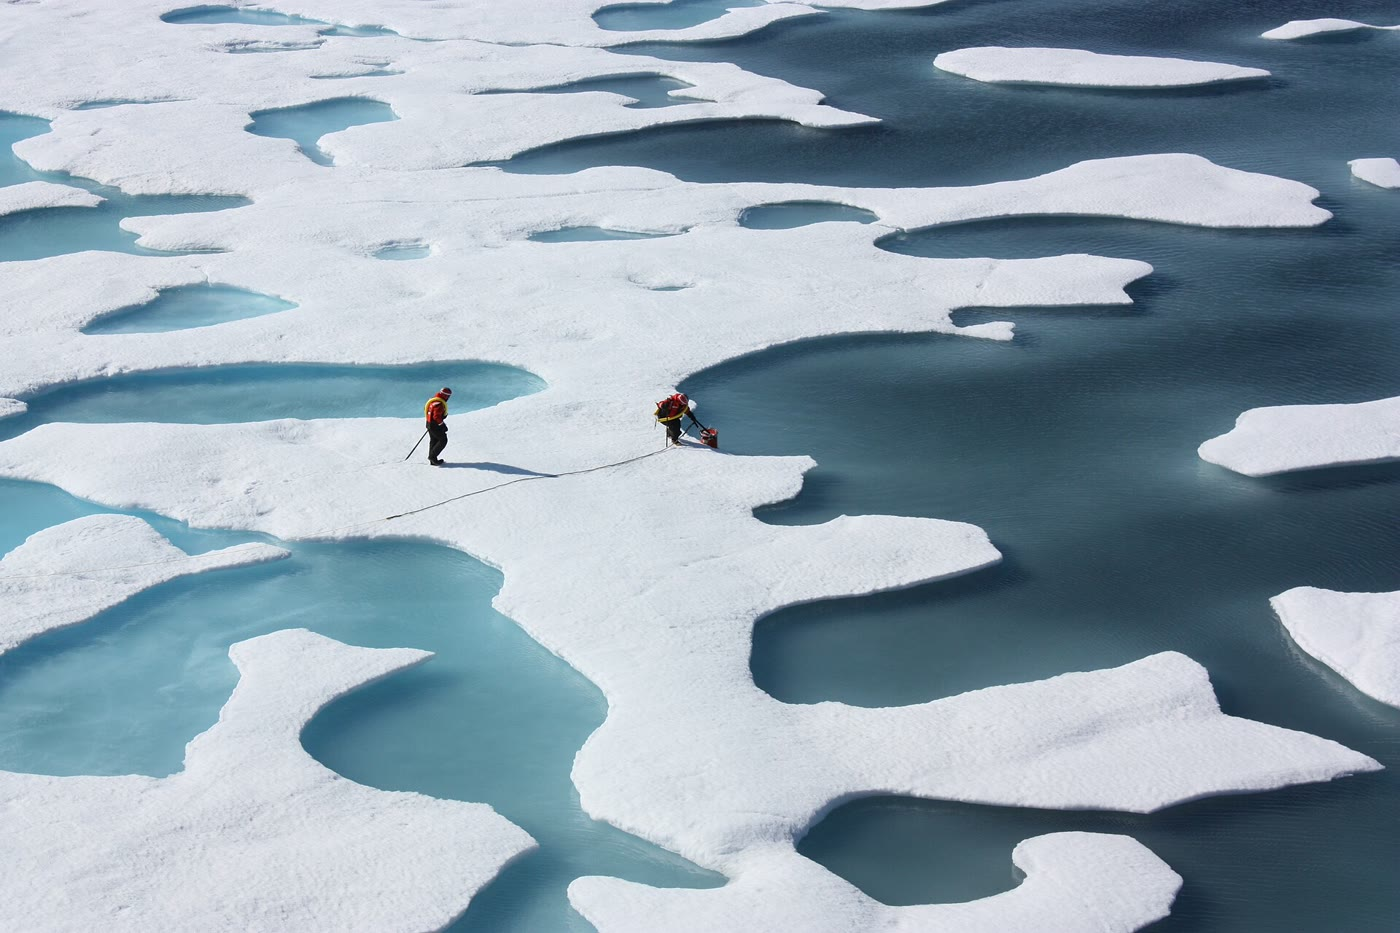
\includegraphics[width=0.78\linewidth]{images/book2/g10-nasa-melt-ponds.jpg}

{\small جليد بحري في المحيط المتجمد الشمالي في يوليو، تحت شمس لا تغرب: جليد أبيض،
وبرك من ماء الذوبان على سطحه، والبحر المكشوف القاتم بين الطوافات. عالمتان تأخذان
عينات من البرك. الصورة: مركز غودارد لرحلات الفضاء التابع لناسا، 2011 (ملك
عام).}
\end{omfigure}

\begin{recall}
تنشأ الفصول من ميل محور الأرض، \qty{23.44}{\degree} عن العمودي على مستوي
مدارها: ففي يونيو يميل نصف الكرة الشمالي نحو الشمس، فتعلو الشمس أكثر في سمائه
وتبقى فوقه مدة أطول (كتب الفيزياء، والكتاب 1). وقد مرّت بنا في
\cref{ch:g10:habitable-planet} الإشعاعية على مسافة الأرض، $S_0 = \qty{1361}{W/m^2}$،
\omterm{def:g10:earth-energy-budget:albedo}{وألبيدو} بوند لكوكب \omterm{def:g10:habitable-planet:equilibrium-temperature}{ودرجة حرارة توازنه}.
وتمتص غازات الدفيئة جزءًا من الأشعة تحت الحمراء التي يطلقها السطح (كتب
الكيمياء). ويصعد الهواء الدافئ ويهبط الهواء البارد، فيدور الهواء في خلايا حمل
ويحرّك الرياح العامة (الكتاب 1، الصف 8). وتصنع النباتات والطحالب وبعض البكتيريا
سكريات من ثاني أكسيد الكربون والماء بطاقة الضوء: إنه التركيب الضوئي (كتب
الأحياء).
\end{recall}

\section{ضوء الشمس الوارد}

ترى الشمس الأرض قرصًا. ففي كل ثانية، تعترض الأرض ضوء الشمس الساقط على قرص نصف
قطره $R$، أي نصف قطرها هي؛ لكن هذا الضوء يتوزع على كل نقاط كرة، نصفها في
الليل.

\begin{proposition}[ربع الثابت الشمسي]\label{prop:g10:earth-energy-budget:quarter}
إذا حُسب المتوسط على سطح الأرض كله وعلى الليل والنهار، فإن قدرة ضوء الشمس الواصل
إلى أعلى الغلاف الجوي هي
\[
  \frac{S_0}{4} = \frac{1361}{4} \approx \qty{340}{W/m^2}.
\]
\end{proposition}

\begin{proof}
تعترض الأرض ضوء الشمس العابر لقرص مساحته $\pi R^2$ عمودي على الأشعة، أي
قدرة $S_0\,\pi R^2$. وبتوزيعها على مساحة الكرة، $4\pi R^2$، نحصل على
$S_0\,\pi R^2/(4\pi R^2) =
S_0/4$ لكل متر مربع.
\end{proof}
% ledger: earth:TSI, ipcc:budget-toa

\begin{omfigure}
\begin{tikzpicture}[font=\small, >={Stealth[length=2mm]}]
  \foreach \y in {-1.2,-0.8,...,1.21}
    \draw[->, omProp!80!black] (-3.4,\y) -- (-1.75,\y);
  \node[anchor=south, font=\footnotesize, align=center] at (-2.6,1.35) {\foreignlanguage{arabic}{ضوء الشمس،}\\\foreignlanguage{arabic}{$S_0$ لكل \babelsublr{m$^2$}}};
  \draw[fill=omProp!15, draw=omProp!80!black] (-1.6,0) ellipse (0.18 and 1.3);
  \node[anchor=north, font=\footnotesize, align=center] at (-1.6,-1.4) {قرص\\$\pi R^2$};
  \shade[ball color=omDef!35] (1.2,0) circle (1.3);
  \fill[black, opacity=0.35] (1.2,1.3) arc (90:-90:1.3) arc (-90:90:0.35 and 1.3);
  \draw[omDef!80!black] (1.2,0) circle (1.3);
  \draw[dashed, black!50] (1.2,-1.3) arc (-90:90:0.35 and 1.3);
  \draw[<->] (1.2,0) -- node[above, font=\footnotesize] {$R$} (2.5,0);
  \node[anchor=west, font=\footnotesize, align=left] at (2.8,0.7) {\foreignlanguage{arabic}{كرة $4\pi R^2$:}\\\foreignlanguage{arabic}{نصفها في النهار،}\\\foreignlanguage{arabic}{ونصفها في الليل}};
  \node[anchor=west, font=\footnotesize, align=left] at (2.8,-0.75) {\foreignlanguage{arabic}{المتوسط:}\\$S_0\pi R^2/4\pi R^2 = S_0/4$};
\end{tikzpicture}

{\small تعترض الأرض ضوء الشمس الساقط على قرص نصف قطره هو نصف قطرها، لكنها
توزعه على مساحة كرة أكبر بأربع مرات: ففي المتوسط يتلقى كل متر مربع من أعلى الغلاف
الجوي ربع الثابت
الشمسي.}
\end{omfigure}

يخفي المتوسط فروقًا كبيرة من مكان إلى آخر. فحزمة ضوء الشمس التي تضرب الأرض
مائلة تنتشر على مساحة أكبر من حزمة تضربها عموديًا.

\begin{proposition}[ضوء الشمس على سطح أفقي]\label{prop:g10:earth-energy-budget:height}
حين تكون الشمس على ارتفاع $h$ فوق الأفق، يتلقى متر مربع أفقي في أعلى الغلاف
الجوي القدرة $S_0 \sin h$.
\end{proposition}

\begin{proof}
لنأخذ حزمة من ضوء الشمس مقطعها \qty{1}{m^2}، مربع الشكل، تحمل
$S_0$. أثرها على الأرض مستطيل أحد ضلعيه \qty{1}{m}
والآخر طوله $\ell$ في اتجاه ميل الأشعة. وفي المثلث القائم الذي يكوّنه ذلك
الضلع والشعاع ومقطع الحزمة، تكون الزاوية عند الأرض $h$ و$\sin h = 1/\ell$.
فقدرة الحزمة تتوزع على $\ell$ مترًا مربعًا: أي $S_0/\ell = S_0 \sin h$ لكل متر
مربع.
\end{proof}

\begin{omfigure}
\begin{tikzpicture}[font=\small, >={Stealth[length=2mm]}]
  \fill[omExo!15] (-0.3,-0.5) rectangle (6.3,0);
  \draw[thick] (-0.3,0) -- (6.3,0);
  \foreach \s in {0,0.3,...,1.21}
    \draw[->, omProp!80!black] ({0.6+\s/sin(35)+3.2*cos(35)},{3.2*sin(35)}) -- ({0.6+\s/sin(35)+0.02*cos(35)},{0.02*sin(35)});
  \draw[omProp!80!black, thick] (0.6,0) -- ({0.6+1.2/sin(35)},0);
  \draw (0.6,0) ++(1.6,0) arc (0:35:1.6);
  \node[font=\footnotesize] at ({0.6+1.85*cos(17)},{1.85*sin(17)}) {$h$};
  \draw[<->] (0.6,-0.25) -- node[below, font=\footnotesize] {$\ell = 1/\sin h$} ({0.6+1.2/sin(35)},-0.25);
  \node[anchor=south west, font=\footnotesize, align=left] at (4.35,1.95) {حزمة\\مقطعها\\\babelsublr{\qty{1}{m^2}}};
\end{tikzpicture}

{\small ضوء الشمس الواصل على ارتفاع $h$ فوق الأفق: تغطي الحزمة نفسها
$1/\sin h$ مترًا مربعًا من الأرض الأفقية، فيتلقى كل متر مربع $S_0 \sin h$.
وكلما انخفضت الشمس، ضعف ضوؤها على
الأرض.}
\end{omfigure}

يتغير ارتفاع الشمس على مدى اليوم، ويتغير طول النهار مع الفصول؛ وكلاهما يدخل في
الطاقة التي يتلقاها مكان ما.

\begin{definition}[الإشماس]\label{def:g10:earth-energy-budget:insolation}
\emph{الإشماس}\index{إشماس} في مكان ما هو قدرة ضوء الشمس التي يتلقاها متر مربع
أفقي في أعلى الغلاف الجوي فوقه. ومتوسطه على ساعات اليوم الأربع والعشرين هو
\emph{متوسط الإشماس اليومي}؛ ومتوسطه على سنة هو \emph{متوسط الإشماس السنوي}؛
ويقاس كلاهما بالوحدة \unit{W/m^2}.
\end{definition}

يتطلب حساب المتوسط اليومي معرفة ارتفاع الشمس في كل لحظة من اليوم، وهذا يستعمل
رياضيات تتجاوز هذا الكتاب؛ وقد أجراه الحاسوب الذي رسم المنحنيات أدناه. وثمة
حالتان بسيطتان. فعلى خط الاستواء في أحد الاعتدالين، تشرق الشمس من الشرق تمامًا،
وتمر فوق الرأس عند الظهيرة، وتغرب في الغرب تمامًا بعد اثنتي عشرة ساعة؛ ومتوسط
ذلك على أربع وعشرين ساعة يعطي $S_0/\pi \approx \qty{433}{W/m^2}$ (نقبله). أما
عند القطب الشمالي فتدور الشمس ببساطة في السماء على ارتفاع ثابت، وهذا ما يستعمله
المثال التالي.

\begin{example}[القطب في يونيو]\label{ex:g10:earth-energy-budget:pole}
% ledger: earth:TSI, earth:obliquity (values computed in figdata/grade-10/energy_budget.py)
في الانقلاب الصيفي في يونيو تبقى الشمس على ارتفاع \qty{23.44}{\degree} فوق أفق
القطب الشمالي طوال اليوم. ومتوسط \omterm{def:g10:earth-energy-budget:insolation}{الإشماس} اليومي هناك $1361
\times \sin 23.44^\circ \approx \qty{541}{W/m^2}$؛ وعلى مدى أربع وعشرين ساعة
يبلغ ذلك $541 \times 24 \approx \qty{13000}{Wh}$، أي \qty{13.0}{kWh} لكل متر
مربع. وفي اليوم نفسه يتلقى خط الاستواء متوسطًا يوميًا قدره
\qty{397}{W/m^2}، أي \qty{9.5}{kWh} لكل متر مربع: فالشمس تعلو هناك أكثر عند
الظهيرة، لكنها تغيب اثنتي عشرة ساعة.
\end{example}

\begin{omfigure}
\begin{tikzpicture}
\begin{axis}[omrecord, width=0.92\linewidth, height=6.4cm, xmin=1, xmax=365,
  ymin=0, ymax=600, ylabel={\foreignlanguage{arabic}{متوسط الإشماس اليومي \babelsublr{(\unit{W/m^2})}}},
  xtick={1,32,60,91,121,152,182,213,244,274,305,335},
  xticklabels={1,2,3,4,5,6,7,8,9,10,11,12}, xlabel={\foreignlanguage{arabic}{الشهر}},
  legend style={at={(0.5,1.02)}, anchor=south, legend columns=4, font=\footnotesize, draw=none},
  tick label style={font=\small}, label style={font=\small}]
\addplot[omThm!85!black, thick] table[x=day, y=Q0] {figdata/out/grade-10-energy_budget-daily.dat};
\addlegendentry{خط الاستواء}
\addplot[omProp!90!black, thick, densely dashed] table[x=day, y=Q30] {figdata/out/grade-10-energy_budget-daily.dat};
\addlegendentry{\foreignlanguage{arabic}{\mbox{\textdir TLT\qty{30}{\degree}} ش}}
\addplot[omMeth!85!black, thick, dashdotted] table[x=day, y=Q60] {figdata/out/grade-10-energy_budget-daily.dat};
\addlegendentry{\foreignlanguage{arabic}{\mbox{\textdir TLT\qty{60}{\degree}} ش}}
\addplot[omDef!85!black, thick] table[x=day, y=Q90] {figdata/out/grade-10-energy_budget-daily.dat};
\addlegendentry{القطب الشمالي}
\end{axis}
\end{tikzpicture}

{\small متوسط \omterm{def:g10:earth-energy-budget:insolation}{الإشماس} اليومي في أعلى الغلاف الجوي على مدى السنة عند أربع دوائر عرض
في نصف الكرة الشمالي (محسوب لمدار دائري، من الثابت الشمسي وميل المحور)؛ والأشهر
مرقّمة من 1 (يناير) إلى 12 (ديسمبر). لا يتلقى القطب شيئًا نصف السنة، ويتلقى حول
الانقلاب الصيفي في يونيو أكثر من أي مكان آخر.}
\end{omfigure}

\begin{remark}[قراءة المنحنيات]\label{rem:g10:earth-energy-budget:curves}
يكاد \omterm{def:g10:earth-energy-budget:insolation}{إشماس} خط الاستواء لا يتغير: قيمتان عظميان ضحلتان عند الاعتدالين، حين تمر
الشمس فوق الرأس عند الظهيرة. وكلما اتجهنا شمالًا، كبر التأرجح بين الصيف والشتاء.
وفيما وراء $90^\circ - 23.44^\circ = \qty{66.56}{\degree}$ نحو القطب تبقى الشمس
تحت الأفق في الانقلاب الشتوي في ديسمبر: إنها الليلة القطبية. ومن نحو 10 مايو إلى
نهاية يوليو يتلقى كل من القطب الشمالي ودائرة العرض \qty{60}{\degree} ش أكثر مما
يتلقاه خط الاستواء.
\end{remark}

أما على مدى سنة كاملة فتتغير الصورة: إذ ينخفض متوسط \omterm{def:g10:earth-energy-budget:insolation}{الإشماس} السنوي، المرسوم في
قسم الفائض والعجز أدناه، من \qty{416}{W/m^2} عند خط الاستواء إلى \qty{172}{W/m^2}
عند القطبين. فوفرة الصيف في المناطق القطبية لا تعوّض ليلها الطويل وشمسها
المنخفضة.

\begin{remark}[البعد عن الشمس لا يصنع الفصول]\label{rem:g10:earth-energy-budget:distance}
% ledger: earth:peri, earth:aph, nasa:earth-perihelion-longitude (ratios computed)
مدار الأرض ليس دائرة تمامًا: فبعدها عن الشمس يتغير بين \num{147.1} و\num{152.1}
مليون كيلومتر، أي بنحو \qty{3}{\percent}، فيتغير ضوء الشمس بنحو
\qty{7}{\percent}. وتكون الأرض أقرب ما تكون إلى الشمس في أوائل يناير، في منتصف
الشتاء الشمالي. وتهمل المنحنيات أعلاه هذا التغير الصغير؛ فالفصول تنشأ من ميل
المحور، وهي متعاكسة في نصفي الكرة.
\end{remark}

\section{الألبيدو}

جزء من ضوء الشمس الواصل إلى الأرض لا يسخّن شيئًا أبدًا: فالسحب والهواء والثلج
والبحر ترده إلى الفضاء.

\begin{definition}[الألبيدو]\label{def:g10:earth-energy-budget:albedo}
\emph{الألبيدو}\index{ألبيدو} لسطح ما هو الكسر الذي يعكسه من ضوء الشمس الساقط
عليه، وهو عدد بين 0 (امتصاص الضوء كله) و1 (عكسه كله). وألبيدو بوند في
\cref{ch:g10:habitable-planet} هو ألبيدو كوكب مأخوذ ككل.
\end{definition}

\begin{omfigure}
\begin{tikzpicture}[font=\small, x=9cm, y=0.55cm]
  \foreach \lab/\lo/\hi/\n in {ثلج حديث/0.80/0.90/8, جليد بحري/0.50/0.70/7,
      رمل صحراوي/0.40/0.40/6, الأرض كلها/0.30/0.30/5, عشب أخضر/0.25/0.25/4,
      تربة عارية/0.17/0.17/3, غابة صنوبرية/0.08/0.15/2, محيط مكشوف/0.06/0.06/1,
      إسفلت حديث/0.04/0.04/0} {
    \fill[omDef!45] (0,\n-0.32) rectangle (\lo,\n+0.32);
    \ifdim\hi pt>\lo pt
      \fill[omDef!18] (\lo,\n-0.32) rectangle (\hi,\n+0.32);
      \draw[omDef!80!black] (\lo,\n-0.32) rectangle (\hi,\n+0.32);
    \fi
    \draw[omDef!80!black] (0,\n-0.32) rectangle (\lo,\n+0.32);
    \node[anchor=east, font=\footnotesize] at (-0.01,\n) {\lab};
  }
  \draw (0,-0.6) -- (1,-0.6);
  \foreach \x in {0,0.2,...,1.01}
    \draw (\x,-0.6) -- (\x,-0.75) node[below, font=\footnotesize] {\pgfmathprintnumber[fixed, precision=1]{\x}};
  \node[font=\footnotesize] at (0.5,-2.0) {الألبيدو};
\end{tikzpicture}

{\small \omterm{def:g10:earth-energy-budget:albedo}{الألبيدو} المعتاد لسطوح مختلفة وللأرض كلها؛ والجزء الباهت من العمود هو
المجال المعتاد. البيانات: جامعة كولورادو بولدر، بعثة MOSAiC؛ المركز الوطني
لبيانات الثلج والجليد.}
\end{omfigure}
% ledger: albedo:surfaces, nsidc:albedo-ice

يرد الثلج الحديث معظم الضوء الذي يتلقاه، أما المحيط المكشوف فلا يرد منه شيئًا
تقريبًا. ولهذا يحتفظ الجليد البحري في الصورة الافتتاحية ببرودته طوال الصيف
القطبي: فالثلج الذي يعلوه يعكس ما يصل إلى تسعة أعشار ضوء الشمس، بينما يمتص الماء
القاتم بين الطوافات نحو 94 في المئة منه. وحين يذوب الجليد، يحل محله ماء قاتم يمتص
من ضوء الشمس أكثر، فيذيب مزيدًا من الجليد: إنها حلقة تعزّز نفسها يزنها
\cref{ch:g12:climate-change} بين التغذيات المرتدة في المناخ.

\begin{omfigure}
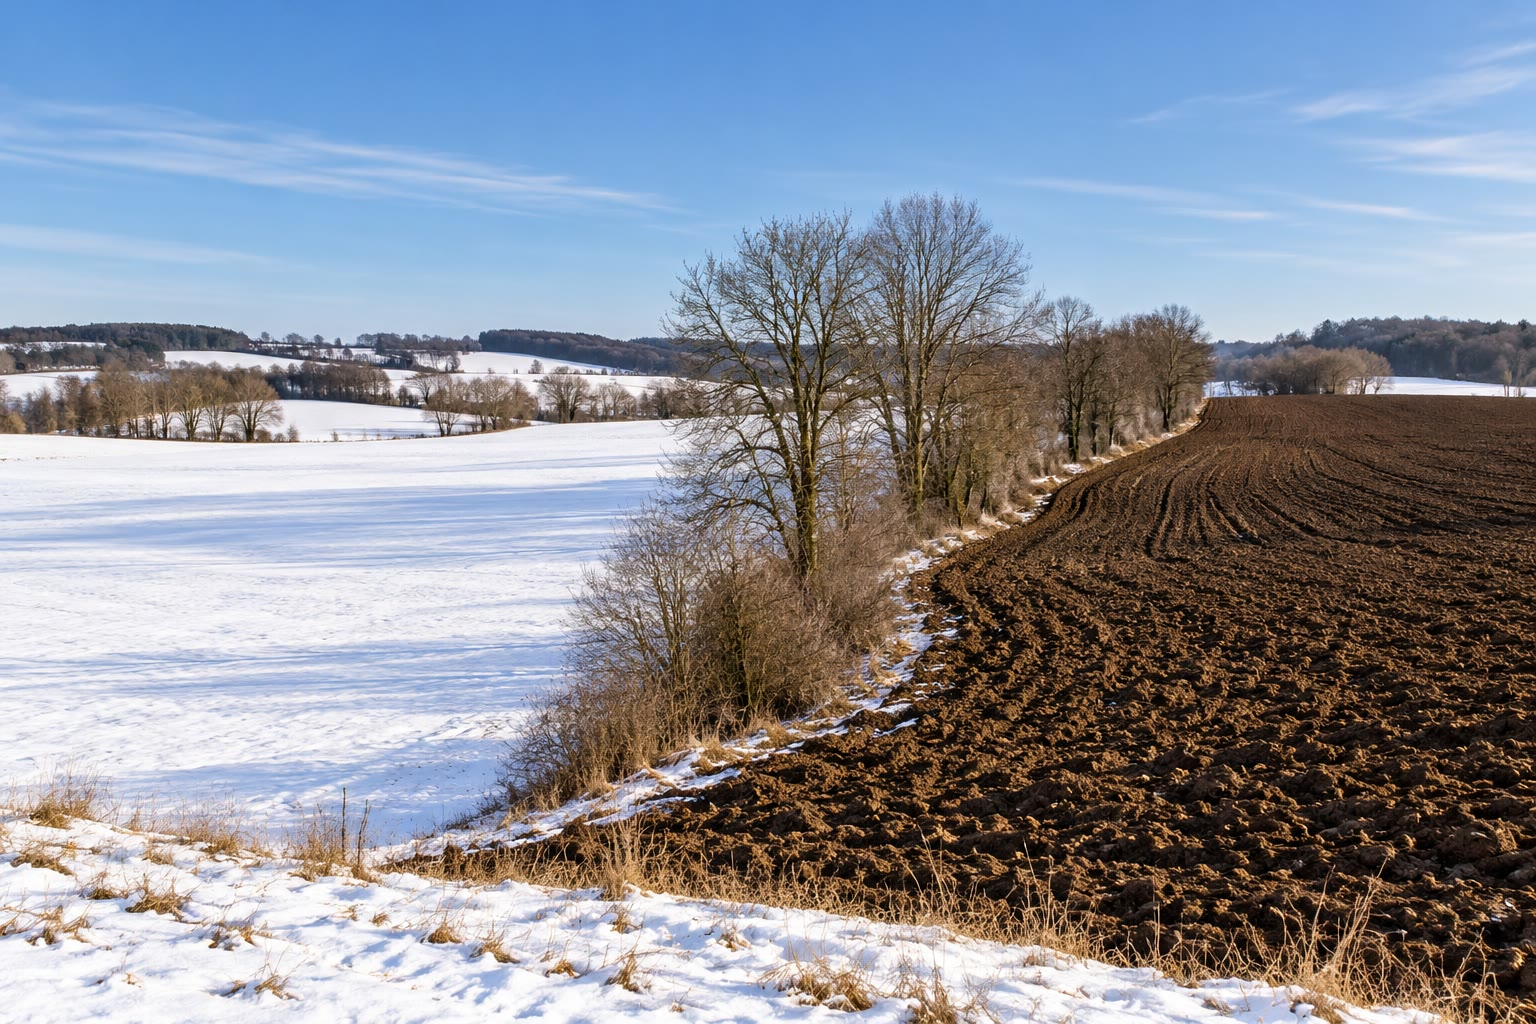
\includegraphics[width=0.7\linewidth]{images/book2/ai/g10-snow-and-ploughed-field.jpg}

{\small صباح شتوي بعد بضعة أيام مشمسة: ما زال الثلج يغطي المرج، لكنه ذاب على الحقل
المحروث القاتم، الذي يمتص من ضوء الشمس قدرًا أكبر
بكثير.}
\end{omfigure}

أما للأرض ككل، فتقيس الأقمار الصناعية ضوء الشمس المنعكس إلى الفضاء مباشرة: في
المتوسط \qty{100}{W/m^2} من \qty{340}{W/m^2} الواصلة، أي \omterm{def:g10:earth-energy-budget:albedo}{ألبيدو} قدره
$100/340 \approx 0.29$. والسحب هي العاكس الرئيس: فالقياسات نفسها، بعد إزالة
السحب حسابيًا، لا تعطي إلا
\qty{53}{W/m^2} منعكسة.
% ledger: ipcc:budget-toa, ipcc:budget-clearsky, earth:albedo

\begin{example}[ضوء الشمس الذي تمتصه الأرض]\label{ex:g10:earth-energy-budget:absorbed}
% ledger: earth:TSI, earth:albedo, earth:Rmean (computed in figdata/grade-10/energy_budget.py)
مع \omterm{def:g10:earth-energy-budget:albedo}{ألبيدو} بوند قدره 0.294، يمتص كل متر مربع في المتوسط $340
\times (1 - 0.294) \approx \qty{240}{W/m^2}$. وعلى الكرة كلها، ومساحتها
$4\pi R^2 = 4\pi \times (\qty{6.371e6}{m})^2 \approx \qty{5.10e14}{m^2}$، تمتص
الأرض $240 \times 5.10\times10^{14} \approx \qty{1.22e17}{W}$ من
ضوء الشمس: وهذه القدرة تحرّك الرياح والتيارات المحيطية ودورة
الماء.
\end{example}

\section{ميزانية الطاقة العالمية}

إلى أين تذهب هذه القدرة، \qty{240}{W/m^2}؟ تعطي اليوم قياساتُ الأقمار الصناعية، وقياسات
الأجهزة على الأرض وعلى السفن، مقرونةً بنماذج الغلاف الجوي، جوابًا متسقًا، متوسطًا
على الكرة الأرضية وعلى عدة سنوات. ويلخصه التقييم العلمي لعام 2021 في المخطط أدناه،
ويقرر أن المركّبات المتوسطة العالمية صارت معروفة بدقة أكبر، في أعلى الغلاف الجوي
وعند السطح (\emph{بثقة
عالية}).
% ledger: ipcc:budget-confidence

\begin{definition}[ميزانية الطاقة]\label{def:g10:earth-energy-budget:energy-budget}
\emph{ميزانية الطاقة}\index{ميزانية الطاقة} لنظام ما --- الأرض كلها، أو سطحها،
أو غلافها الجوي --- هي حساب كل الطاقة الداخلة إليه والخارجة منه، ويُعطى كل تدفق
بوصفه قدرة متوسطة لكل متر مربع من سطح الأرض. وتكون الميزانية \emph{متوازنة} حين
يساوي ما يدخل ما يخرج؛ وإلا فإن النظام يكتسب طاقة أو يفقدها فيسخن أو
يبرد.
\end{definition}

ويفقد السطح أيضًا طاقة من دون أي إشعاع: فالماء يتبخر من البحر ومن الأوراق،
والأرض تدفئ الهواء الملامس لها.

\begin{definition}[الحرارة الكامنة؛ الحرارة المحسوسة]\label{def:g10:earth-energy-budget:latent-heat}
\emph{الحرارة الكامنة}\index{حرارة كامنة} لمادة ما هي الطاقة التي تمتصها حين
تتغير حالتها دون أن تتغير درجة حرارتها --- بالانصهار أو التبخر --- وتعيدها حين
تعود إلى حالتها الأولى. وهي للماء المتبخر عند \qty{15}{\degreeCelsius} نحو
\qty{2.47}{MJ} لكل كيلوغرام. وفي \omterm{def:g10:earth-energy-budget:energy-budget}{ميزانية الطاقة}، \emph{تدفق الحرارة الكامنة}
هو الطاقة التي يأخذها التبخر من السطح ويحررها بخار الماء في الهواء حيث يتكاثف
سحبًا. أما تدفق \emph{الحرارة المحسوسة}\index{حرارة محسوسة}
فهو الطاقة التي ينقلها السطح إلى الهواء الملامس له فيدفئه، ويحملها الهواء الصاعد
نحو الأعلى.
\end{definition}
% ledger: nist:water-latent

\begin{omfigure}
\begin{tikzpicture}[font=\footnotesize, >={Stealth[length=2.2mm, width=2mm]}, line width=1.4pt]
  % layers
  \fill[omDef!8] (0,0.5) rectangle (12.8,4.5);
  \fill[omExo!35] (0,0) rectangle (12.8,0.5);
  \draw[thin, black!60] (0,0.5) -- (12.8,0.5);
  \draw[thin, black!60, dashed] (0,4.5) -- (12.8,4.5);
  \node[anchor=east, black!70, align=right] at (-0.1,5.4) {الفضاء};
  \node[anchor=east, black!70, align=right] at (-0.1,4.5) {أعلى الغلاف\\الجوي};
  \node[anchor=east, black!70, align=right] at (-0.1,2.5) {الغلاف الجوي};
  \node[anchor=east, black!70, align=right] at (-0.1,0.25) {السطح};
  \pic[scale=0.7, transform shape] at (4.3,3.0) {puffycloud};
  \pic[scale=0.7, transform shape] at (6.2,3.0) {puffycloud};
  % sunlight
  \draw[->, omProp!90!black] (1.0,6.1) -- (1.0,0.52);
  \draw[->, omProp!90!black] (1.0,3.0) -- (1.6,3.0);
  \node[anchor=west, align=left] at (1.65,3.0) {\foreignlanguage{arabic}{\mbox{\textdir TLT 80} يمتصها}\\\foreignlanguage{arabic}{الهواء}};
  \node[anchor=west] at (1.05,1.3) {185};
  \draw[->, omProp!55] (4.3,3.7) -- (4.3,6.1);
  \node[anchor=east] at (4.25,5.0) {75};
  \draw[->, omProp!55] (5.25,0.52) -- (5.25,6.1);
  \node[anchor=west] at (5.3,1.2) {25};
  % heat
  \draw[->, omMeth!80!black] (6.2,0.52) -- (6.2,2.95);
  \draw[->, omMeth!80!black] (7.8,0.52) -- (7.8,2.0);
  % infrared
  \draw[->, omThm!80!black] (9.2,0.52) -- (9.2,4.0);
  \draw[->, omThm!80!black] (10.7,3.4) -- (10.7,6.1);
  \draw[->, omThm!50] (12.1,4.0) -- (12.1,0.52);
  % words above the top of the atmosphere
  \node[anchor=south, align=center] at (1.0,6.15) {340\\واردة};
  \node[anchor=south, align=center] at (4.78,6.15) {100\\منعكسة};
  \node[anchor=south, align=center] at (7.7,5.0) {اختلال التوازن\\\foreignlanguage{arabic}{$+0.7$ ممتصة}};
  \node[anchor=south, align=center] at (10.7,6.15) {\foreignlanguage{arabic}{\mbox{\textdir TLT 239} تحت حمراء}\\نحو الفضاء};
  % words below the surface
  \node[anchor=north, align=center] at (1.0,-0.05) {160\\ممتصة};
  \node[anchor=north, align=center] at (6.2,-0.05) {82\\حرارة\\كامنة};
  \node[anchor=north, align=center] at (7.8,-0.05) {21\\حرارة\\محسوسة};
  \node[anchor=north, align=center] at (9.4,-0.05) {398\\منبعثة};
  \node[anchor=north, align=center] at (12.1,-0.05) {342\\إشعاع\\مرتد};
\end{tikzpicture}

{\small \omterm{def:g10:earth-energy-budget:energy-budget}{ميزانية الطاقة} المتوسطة العالمية للأرض في مطلع القرن الحادي والعشرين،
بالوحدة \unit{W/m^2} متوسطةً على السطح كله. البرتقالي: ضوء الشمس؛ والأخضر: الحرارة
التي يحملها التبخر والهواء الدافئ؛ والأحمر: الأشعة تحت الحمراء. ومن القدرة
المنعكسة، 100، يأتي 25 من السطح و75 من السحب والهواء وغباره. وتشمل الأشعة تحت الحمراء
المتجهة إلى الفضاء جزء انبعاث السطح الذي يفلت مباشرة عبر الهواء. البيانات:
الهيئة الحكومية الدولية المعنية بتغير المناخ، تقرير التقييم السادس، الفريق
العامل الأول، الشكل~7.2.}
\end{omfigure}
% ledger: ipcc:budget-toa, ipcc:budget-surface

\begin{method}[قراءة مخطط ميزانية الطاقة]\label{met:g10:earth-energy-budget:reading}
\begin{enumerate}
  \item اختر النظام: الأرض كلها (خط فوق الغلاف الجوي)، أو السطح، أو الغلاف
        الجوي (الطبقة الواقعة بينهما).
  \item عدّد الأسهم الداخلة إليه واجمعها؛ وعدّد الأسهم الخارجة منه
        واجمعها.
  \item قارن المجموعين. فإذا تساويا في حدود تقريب الأعداد، كان النظام في
        توازن؛ والفرق هو ما يكتسبه (أو يفقده) كل ثانية لكل متر
        مربع.
\end{enumerate}
\end{method}

\begin{proposition}[الميزانية متوازنة]\label{prop:g10:earth-energy-budget:balance}
في حدود تقريب الأرقام، الميزانية في المخطط أعلاه متوازنة للأرض ككل، وللسطح،
وللغلاف الجوي، باستثناء فائض صغير يقارب \qty{0.7}{W/m^2} تمتصه الأرض ولا
تعيده.
\end{proposition}

\begin{proof}
\emph{الأرض كلها:} الداخل 340؛ والخارج $100 + 239 = 339$. \emph{السطح:} الداخل
$160 + 342 = 502$؛ والخارج $82 + 21 + 398 = 501$. وفي الحالتين الفائض،
نحو 1، هو اختلال التوازن 0.7 مقرَّبًا. \emph{الغلاف الجوي:} لنسمِّ $W$ جزء
الأشعة تحت الحمراء من السطح الذي يفلت عبر الهواء إلى الفضاء. يتلقى الهواء
$80 + 82 + 21 + (398 - W) = 581 - W$ ويطلق $342$ نحو الأسفل
و$239 - W$ نحو الأعلى، أي $581 - W$ في المجموع: فهو متوازن، أيًّا كانت $W$.
\end{proof}
% ledger: ipcc:budget-toa, ipcc:budget-surface (closures checked in figdata/grade-10/energy_budget.py)

ويُظهر المخطط أيضًا أثر الدفيئة وهو يعمل. فالسطح يتلقى من الهواء، على شكل أشعة تحت
حمراء، \qty{342}{W/m^2} --- أي أكثر من ضعف ضوء الشمس الذي يمتصه،
\qty{160}{W/m^2}. ولهذا يستطيع أن يطلق \qty{398}{W/m^2}، وهو انبعاث جسم عند نحو
\qty{15}{\degreeCelsius}، بينما لا ترسل الأرض إلى الفضاء إلا
\qty{239}{W/m^2}. وتبني كتب الفيزياء النموذج الذي يربط هذه الأعداد بدرجة الحرارة؛
أما هذا الكتاب فيستعمل التدفقات المقيسة.

\begin{example}[متر من الماء في السنة]\label{ex:g10:earth-energy-budget:evaporation}
% ledger: ipcc:budget-surface, nist:water-latent (computed in figdata/grade-10/energy_budget.py)
يبخّر تدفق \omterm{def:g10:earth-energy-budget:latent-heat}{الحرارة الكامنة}، \qty{82}{W/m^2}، في كل ثانية $82/2.47\times
10^6 \approx \qty{3.3e-5}{kg}$ من الماء لكل متر مربع. وعلى مدى سنة،
$3.16\times10^7$ ثانية، يبلغ ذلك نحو \qty{1050}{kg}، أي طبقة من الماء سماكتها
\qty{1.05}{m} على الأرض كلها. والهواء لا يحمل إلا قليلًا من الماء في كل وقت،
فيعود كله تقريبًا مطرًا وثلجًا: فتدفق \omterm{def:g10:earth-energy-budget:latent-heat}{الحرارة الكامنة} والهطول السنوي على الكوكب
وجهان لدورة الماء
نفسها.
\end{example}

\begin{remark}[اختلال التوازن]\label{rem:g10:earth-energy-budget:imbalance}
% ledger: ipcc:budget-toa, ipcc:heating
يبدو الفائض \qty{0.7}{W/m^2} ضئيلًا بجانب تدفقات من مئات الواطات، لكنه على الأرض
كلها يساوي $0.7 \times 5.10\times10^{14} \approx
\qty{3.6e14}{W}$، يُخزن معظمه في المحيط، الذي يسخن. وهو ليس ثابتًا طبيعيًا: فقد
ازداد في العقود الأخيرة، كما يشرح
\cref{ch:g12:climate-change}.
\end{remark}

\section{الفائض والعجز}

تتوازن الميزانية للأرض ككل، لكن لا عند كل دائرة عرض.

\begin{omfigure}
\begin{tikzpicture}
\begin{axis}[omrecord, width=0.86\linewidth, height=5.6cm, xmin=0, xmax=90,
  ymin=0, ymax=450, xlabel={\foreignlanguage{arabic}{العرض الجغرافي \babelsublr{(\unit{\degree})}}},
  ylabel={\foreignlanguage{arabic}{متوسط الإشماس السنوي \babelsublr{(\unit{W/m^2})}}}, xtick={0,15,...,90},
  tick label style={font=\small}, label style={font=\small}]
\addplot[omThm!85!black, thick] table[x=lat, y=Qann] {figdata/out/grade-10-energy_budget-annual.dat};
\addplot[omDef!80!black, dashed, domain=0:90] {340.25};
\node[anchor=south west, font=\footnotesize, omDef!80!black] at (axis cs:2,343) {\foreignlanguage{arabic}{المتوسط العالمي، 340}};
\node[anchor=south west, font=\footnotesize, omThm!85!black] at (axis cs:62,232) {المتوسط السنوي};
\end{axis}
\end{tikzpicture}

{\small متوسط \omterm{def:g10:earth-energy-budget:insolation}{الإشماس} السنوي في أعلى الغلاف الجوي بحسب العرض الجغرافي (وهو نفسه في
نصفي الكرة؛ محسوب من الثابت الشمسي وميل المحور). وبين خط الاستواء ونحو
\qty{37}{\degree} يتجاوز المتوسط العالمي؛ وفيما وراء ذلك نحو القطب يقصر
عنه.}
\end{omfigure}

تمتص المنطقة المدارية من ضوء الشمس أكثر بكثير مما تمتصه المناطق القطبية، ويوسّع
ألبيدوها المنخفض الفارق. والأشعة تحت الحمراء التي ترسلها إلى الفضاء أكبر أيضًا،
لأنها أدفأ، لكنها تتغير مع العرض الجغرافي أقل بكثير. ونتيجة لذلك، تمتص المناطق
المحيطة بخط الاستواء في المتوسط نحو \qty{200}{W/m^2} أكثر مما تعكسه وتشعه، وتشع
المناطق القريبة من القطبين نحو \qty{200}{W/m^2} أكثر مما
تمتصه.
% ledger: nasaeo:surplus

\begin{definition}[نقل الحرارة نحو القطبين]\label{def:g10:earth-energy-budget:heat-transport}
\emph{نقل الحرارة نحو القطبين}\index{نقل الحرارة نحو القطبين} هو تدفق الطاقة
الذي تحمله حركات الغلاف الجوي والمحيط من المنطقة المدارية نحو القطبين. ويقاس،
عبر دائرة عرض، بالبيتاواط (\qty{1}{PW} = \qty{e15}{W}).
\end{definition}

لولاه لازدادت المنطقة المدارية حرارة والقطبان برودة حتى توازن كل دائرة عرض
ميزانيتها الخاصة. ويقوم الغلاف الجوي بمعظم النقل: هواء دافئ يتجه نحو القطب وهواء
بارد يعود نحو خط الاستواء، وبخار ماء يحرر حرارته الكامنة بعيدًا عن مكان تبخره.
وتحمل التيارات المحيطية الباقي. وتضع التقديرات المستندة إلى القياسات النقلَ
الجوي نحو القطب عند قيمة عظمى تقارب \qty{5.0}{PW} قرب
\qty{43}{\degree} ش، مع قيم مماثلة قرب \qty{40}{\degree} ج؛ ولا يحمل المحيط أكثر
من الغلاف الجوي إلا قرب خط الاستواء، بين
\qty{0}{\degree} و\qty{17}{\degree} ش، وعند \qty{35}{\degree} ش، حيث يكون النقل
الكلي أكبر ما يكون، يحمل الغلاف الجوي \qty{78}{\percent}
منه. ويكون النقل الكلي أكبر ما يكون هناك لأن \qty{35}{\degree} هو تقريبًا موضع
تحوّل الفائض إلى عجز: فنحو خط الاستواء يظل النقل يجمع فائض كل دائرة عرض يعبرها؛
ونحو القطب تستمد منه كل دائرة عرض.
% ledger: trenberth:transport

\begin{omfigure}
\begin{tikzpicture}[font=\footnotesize, >={Stealth[length=2mm]}]
  \def\R{2.4}
  \begin{scope}
    \clip (0,0) circle (\R);
    \fill[omThm!22] (-\R,{-\R*sin(35)}) rectangle (\R,{\R*sin(35)});
    \fill[omDef!22] (-\R,{\R*sin(35)}) rectangle (\R,\R);
    \fill[omDef!22] (-\R,-\R) rectangle (\R,{-\R*sin(35)});
  \end{scope}
  \draw[thick] (0,0) circle (\R);
  \draw[black!50] (-\R,0) -- (\R,0);
  \foreach \s in {1,-1} \draw[black!40, dashed] ({-\R*cos(35)},{\s*\R*sin(35)}) -- ({\R*cos(35)},{\s*\R*sin(35)});
  \node at (0,0.45) {فائض};
  \node at (0,1.95) {عجز};
  \node at (0,-1.95) {عجز};
  \node[anchor=west, black!60] at (\R+0.05,0) {خط الاستواء};
  \node[anchor=west, black!60] at ({\R*cos(35)+0.05},{\R*sin(35)}) {\foreignlanguage{arabic}{\mbox{\textdir TLT\qty{35}{\degree}} ش}};
  \node[anchor=west, black!60] at ({\R*cos(35)+0.05},{-\R*sin(35)}) {\foreignlanguage{arabic}{\mbox{\textdir TLT\qty{35}{\degree}} ج}};
  \foreach \s in {1,-1} {
    \draw[->, very thick, omProp!90!black] ({-(\R+0.35)*cos(10)},{\s*(\R+0.35)*sin(10)}) arc ({180-10*\s}:{180-70*\s}:{\R+0.35});
    \draw[->, thick, omMeth!80!black] ({-(\R-0.45)*cos(8)},{\s*(\R-0.45)*sin(8)}) arc ({180-8*\s}:{180-55*\s}:{\R-0.45});
  }
  \node[anchor=east, omProp!90!black, align=right] at (-\R-0.75,1.6) {الغلاف الجوي};
  \node[anchor=east, omProp!90!black, align=right] at (-\R-0.75,-1.6) {الغلاف الجوي};
  \node[omMeth!80!black] at (-1.25,0.62) {المحيط};
  \node[omMeth!80!black] at (-1.25,-0.62) {المحيط};
\end{tikzpicture}

{\small بين نحو \qty{35}{\degree} ج و\qty{35}{\degree} ش تمتص الأرض طاقة أكثر
مما تشع؛ وفيما وراء دائرتي العرض هاتين نحو القطبين تشع أكثر مما تمتص. ويحمل
الغلاف الجوي (البرتقالي) والمحيط (الأخضر) الفائض نحو القطبين. رسم تخطيطي: عرض
الأسهم ليس بمقياس رسم.}
\end{omfigure}

هذا النقل هو محرك الطقس. فخلايا الحمل والرياح العامة في الكتاب 1، وعواصف
\cref{ch:g10:storms-and-cyclones}، والتيارات المحيطية الكبرى في
\cref{ch:g10:layered-ocean}، كلها تنقل الحرارة من حيث تعطي الشمس أكثر مما ينبغي
إلى حيث تعطي أقل مما ينبغي.

\section{أين تذهب الطاقة}

تنتهي كل طاقة ضوء الشمس التي تمتصها الأرض تقريبًا حرارةً: فهي تدفئ الأرض والبحر
والهواء، وتبخّر الماء، وتحرّك الرياح والتيارات، ثم تغادر من جديد على شكل ضوء تحت
أحمر. أما جزء ضئيل منها فيسلك طريقًا آخر: إذ يخزنه التركيب الضوئي في الروابط
الكيميائية للسكريات، ومنها في كل المادة الحية على الكوكب.

\begin{example}[حصة التركيب الضوئي]\label{ex:g10:earth-energy-budget:photosynthesis}
% ledger: field:npp, nist:glucose-combustion, earth:Rmean (computed in figdata/grade-10/energy_budget.py)
تخزن النباتات على اليابسة والطحالب في البحر، بعد سد حاجاتها الخاصة، نحو
\num{105} مليار طن من الكربون في مادة حية جديدة كل سنة، نصفها تقريبًا على
اليابسة ونصفها في المحيط: ويسميها علماء البيئة الإنتاج الأولي الصافي للكوكب.
واحتراق مول من الغلوكوز،
\ce{C6H12O6}، الذي يحوي ستة مولات من الكربون، أي \qty{72}{g}، يحرر
\qty{2805}{kJ}: أي نحو \qty{38.9}{kJ} لكل غرام من الكربون. والطاقة المخزنة
كل سنة هي $1.049\times10^{17}\,\unit{g} \times \qty{38.9e3}{J/g} \approx
\qty{4.1e21}{J}$، أي قدرة قدرها $4.1\times10^{21}/3.16\times10^{7} \approx
\qty{1.3e14}{W}$. ومقارنةً بالقدرة \qty{1.22e17}{W} من ضوء الشمس التي تمتصها
الأرض، يمثل هذا نحو \qty{0.1}{\percent}.
\end{example}

\begin{remark}[حصة صغيرة، ودور كبير]\label{rem:g10:earth-energy-budget:life}
جزء من ألف من ضوء الشمس الممتص يغذي كل الحياة على الأرض تقريبًا، وبقايا النباتات
والطحالب المدفونة على مدى مئات ملايين السنين تكوّن الفحم والنفط والغاز الطبيعي
(\cref{ch:g11:fossil-fuel-geology}). أما باقي ضوء الشمس --- أكثر من 99.9 في
المئة --- فيبقي الكوكب دافئًا ويحرّك هواءه وماءه وطقسه.
\end{remark}

\section{تمارين}

\begin{exercise}[$\star$]\label{exo:g10:earth-energy-budget:1}
عرّف \omterm{def:g10:earth-energy-budget:insolation}{الإشماس} في مكان ما \omterm{def:g10:earth-energy-budget:albedo}{وألبيدو} سطح ما. أيهما يعكس الكسر الأكبر من ضوء الشمس:
الثلج الحديث أم المحيط المكشوف؟
\end{exercise}

\begin{exercise}[$\star$]\label{exo:g10:earth-energy-budget:2}
باستعمال مخطط \omterm{def:g10:earth-energy-budget:energy-budget}{ميزانية الطاقة} في هذا الفصل، أعطِ بالنسب المئوية من
\qty{340}{W/m^2} الواصلة إلى أعلى الغلاف الجوي الحصة المنعكسة إلى الفضاء،
والحصة التي يمتصها الهواء، والحصة التي يمتصها
السطح.
\end{exercise}

\begin{exercise}[$\star$]\label{exo:g10:earth-energy-budget:3}
شمس صيفية توصل \qty{800}{W/m^2} إلى الأرض. ما القدرة التي يمتصها متر مربع إذا
كان مغطى بإسفلت حديث (\omterm{def:g10:earth-energy-budget:albedo}{ألبيدو} 0.04)، وإذا كان مغطى بثلج حديث (\omterm{def:g10:earth-energy-budget:albedo}{ألبيدو}
0.85)؟
\end{exercise}

\begin{exercise}[$\star$]\label{exo:g10:earth-energy-budget:4}
أيهما يحمل من سطح الأرض طاقة أكثر: التبخر أم تدفئة الهواء الملامس للأرض؟ وصِف في
جملتين كيف تبلغ الطاقة التي يأخذها التبخر من البحر الهواءَ المرتفع
فوقه.
\end{exercise}

\begin{exercise}[$\star$]\label{exo:g10:earth-energy-budget:5}
فسّر لماذا يكون متوسط \omterm{def:g10:earth-energy-budget:insolation}{الإشماس} اليومي صفرًا عند القطب الشمالي في ديسمبر،
وأعطِ دائرة العرض التي يحدث ذلك وراءها في الانقلاب الشتوي في ديسمبر.
\end{exercise}

\begin{exercise}[$\star\star$]\label{exo:g10:earth-energy-budget:6}
باستعمال \cref{prop:g10:earth-energy-budget:height}، احسب القدرة التي يتلقاها
متر مربع أفقي في أعلى الغلاف الجوي حين تكون الشمس على ارتفاع
\qty{90}{\degree} و\qty{30}{\degree} و\qty{10}{\degree} فوق الأفق.
وعند أي ارتفاع للشمس يتلقى المتر المربع نصف $S_0$؟
\end{exercise}

\begin{exercise}[$\star\star$]\label{exo:g10:earth-energy-budget:7}
باتباع \cref{met:g10:earth-energy-budget:reading}، تحقق من ميزانية ضوء
الشمس وحده: من \qty{340}{W/m^2} الواصلة، كم ينعكس، وكم يمتصه الهواء، وكم يمتصه
السطح؟ وهل مجموع الثلاثة 340؟ وتحقق أيضًا من أن ضوء الشمس الواصل إلى السطح،
\qty{185}{W/m^2}، إما أن ينعكس هناك وإما أن
يُمتص.
\end{exercise}

\begin{exercise}[$\star\star$]\label{exo:g10:earth-energy-budget:8}
باستعمال متوسط نصف قطر الأرض \qty{6371}{km}، احسب مساحة القرص الذي يعترض ضوء
الشمس والقدرة التي يعترضها، ثم مساحة الكرة. واستنتج متوسط القدرة لكل متر مربع من
الكرة.
\end{exercise}

\begin{exercise}[$\star\star$]\label{exo:g10:earth-energy-budget:9}
فائض الأرض \qty{0.7}{W/m^2} على مساحة
\qty{5.10e14}{m^2}. ما الطاقة، بالجول، التي تكتسبها الأرض في سنة من
$3.16\times10^7$ ثانية؟
\end{exercise}

\begin{exercise}[$\star\star$]\label{exo:g10:earth-energy-budget:10}
لو أُزيلت السحب حسابيًا، لعكست الأرض
\qty{53}{W/m^2} بدلًا من \qty{100}{W/m^2}، ولأرسلت \qty{267}{W/m^2} من الأشعة
تحت الحمراء إلى الفضاء بدلًا من \qty{239}{W/m^2}. بكم تغيّر السحب ضوء الشمس
الممتص، والأشعة تحت الحمراء المفقودة؟ وهل تدفئ السحب الأرض أم تبردها، في
المحصلة؟
\end{exercise}

\begin{exercise}[$\star\star$]\label{exo:g10:earth-energy-budget:11}
اقرأ منحنيات متوسط \omterm{def:g10:earth-energy-budget:insolation}{الإشماس} اليومي في هذا الفصل. في أي الأشهر يكون متوسط \omterm{def:g10:earth-energy-budget:insolation}{الإشماس}
اليومي عند القطب الشمالي أكبر منه عند خط الاستواء؟ ولماذا يُظهر منحنى خط
الاستواء قيمتين عظميين لا قيمة واحدة؟
\end{exercise}

\begin{exercise}[$\star\star\star$]\label{exo:g10:earth-energy-budget:12}
\omterm{def:g10:earth-energy-budget:latent-heat}{الحرارة الكامنة} لتبخر الماء \qty{2.47}{MJ/kg} وتدفق \omterm{def:g10:earth-energy-budget:latent-heat}{الحرارة الكامنة}
\qty{82}{W/m^2}. احسب سماكة الماء، بالمليمترات، المتبخر من المتر المربع المتوسط
من الأرض كل يوم، وبالأمتار كل سنة (لتر واحد من الماء موزع على متر مربع يكوّن
طبقة سماكتها
\qty{1}{mm}).
\end{exercise}

\begin{exercise}[$\star\star\star$]\label{exo:g10:earth-energy-budget:13}
عند القطب الشمالي تدور الشمس في السماء على ارتفاع يساوي ميلها $\delta$، فيكون
متوسط \omterm{def:g10:earth-energy-budget:insolation}{الإشماس} اليومي هناك $S_0 \sin
\delta$. أوجد الميل الذي يتلقى عنده القطب، في متوسط اليوم، قدر ما يتلقاه خط
الاستواء في أحد الاعتدالين، أي $S_0/\pi$. ويحقق الميل العلاقة
$\sin\delta = \sin 23.44^\circ \times \sin\lambda$، حيث
تزداد الزاوية $\lambda$ بانتظام بمقدار \qty{360}{\degree} في السنة، من
\qty{0}{\degree} عند اعتدال مارس (و\qty{90}{\degree} عند انقلاب
يونيو). فكم يومًا تقريبًا في السنة يتلقى القطب أكثر من
$S_0/\pi$؟
\end{exercise}

\begin{exercise}[$\star\star\star$]\label{exo:g10:earth-energy-budget:14}
افترض أنه في الصيف تذوب مساحة \qty{1e12}{m^2} من الجليد البحري (\omterm{def:g10:earth-energy-budget:albedo}{ألبيدو} 0.6)
ويحل محلها محيط مكشوف (\omterm{def:g10:earth-energy-budget:albedo}{ألبيدو} 0.06)، تحت ضوء شمس متوسطه
\qty{300}{W/m^2} عند السطح. احسب القدرة الإضافية
الممتصة. وقارنها بالقدرة التي يخزنها التركيب الضوئي كله على
الأرض، \qty{1.3e14}{W}، وفسّر لماذا يعزز هذا التبادل بين السطوح
نفسه.
\end{exercise}

\begin{exercise}[$\star\star\star$]\label{exo:g10:earth-energy-budget:15}
بعد الأرض عن الشمس \num{147.1} مليون كيلومتر في أقرب نقطة
و\num{152.1} مليونًا في أبعد نقطة، بمتوسط
\num{149.6} مليونًا، حيث $S_0 = \qty{1361}{W/m^2}$. احسب الإشعاعية الشمسية
عند الطرفين. والفرق قريب من
\qty{90}{W/m^2}؛ أما عند \qty{60}{\degree} ش، فمتوسط \omterm{def:g10:earth-energy-budget:insolation}{الإشماس} اليومي نحو
\qty{490}{W/m^2} في يونيو و\qty{24}{W/m^2} في ديسمبر. فسّر لماذا لا يمكن أن
تكون المسافة سبب الفصول.
\end{exercise}

\section{مسألة: في أثر شعاع من الشمس}

\begin{problem}[{مسألة نهاية الأسبوع --- من ضوء الشمس الذي يبلغ الأرض إلى الحصة
التي تخزنها الحياة}]
\label{pb:g10:earth-energy-budget:1}
% ledger: earth:TSI, earth:Rmean, ipcc:budget-toa, ipcc:budget-surface, ipcc:budget-clearsky, nist:water-latent, field:npp, nist:glucose-combustion (all results computed in figdata/grade-10/energy_budget.py or from the rounded data below)
استعمل $S_0 = \qty{1361}{W/m^2}$، ونصف قطر الأرض $R = \qty{6371}{km}$،
و$\sigma = \qty{5.67e-8}{W.m^{-2}.K^{-4}}$، وسنةً من $3.156\times10^7$
ثانية، وتدفقات مخطط \omterm{def:g10:earth-energy-budget:energy-budget}{ميزانية الطاقة}، وحرارةً كامنة للتبخر قدرها
\qty{2.47}{MJ/kg}، وإنتاجًا أوليًا صافيًا عالميًا قدره
\num{104.9} مليار طن من الكربون في السنة، و\qty{2805}{kJ} تتحرر
باحتراق مول من الغلوكوز (\qty{72.07}{g} من الكربون).

\medskip
\noindent\textbf{الجزء الأول --- هندسة ضوء الشمس.}
\begin{enumerate}
  \item احسب مساحة القرص الذي يعترض ضوء الشمس، $\pi R^2$، بالأمتار
        المربعة.
  \item احسب قدرة ضوء الشمس التي يعترضها.
  \item احسب مساحة سطح الأرض، $4\pi R^2$.
  \item استنتج متوسط القدرة الواصلة لكل متر مربع من أعلى الغلاف
        الجوي.
  \item في أحد الاعتدالين عند الظهيرة، تكون الشمس فوق الرأس على خط الاستواء
        وعلى ارتفاع \qty{30}{\degree} فوق الأفق عند \qty{60}{\degree} ش. فماذا
        يتلقى متر مربع أفقي في كل من المكانين؟
\end{enumerate}

\medskip
\noindent\textbf{الجزء الثاني --- الألبيدو.}
\begin{enumerate}[resume]
  \item احسب \omterm{def:g10:earth-energy-budget:albedo}{ألبيدو} الأرض من القدرة المنعكسة \qty{100}{W/m^2}.
  \item احسب القدرة الممتصة لكل متر مربع وعلى الأرض كلها.
  \item من دون السحب، ينعكس \qty{53}{W/m^2}. فكم يكون \omterm{def:g10:earth-energy-budget:albedo}{الألبيدو}؟ وبأي عامل
        ترفعه السحب؟
  \item احسب \omterm{def:g10:habitable-planet:equilibrium-temperature}{درجة حرارة التوازن} الموافقة للقدرة الممتصة في السؤال 7
        (\cref{ch:g10:habitable-planet})، وقارنها بدرجة حرارة السطح
        \qty{288}{K}.
\end{enumerate}

\medskip
\noindent\textbf{الجزء الثالث --- السطح.}
\begin{enumerate}[resume]
  \item اجمع تدفقات الطاقة الداخلة إلى السطح.
  \item اجمع التدفقات الخارجة منه، وقارن.
  \item كم مرة تفوق الأشعة تحت الحمراء التي يتلقاها السطح من الهواء ضوءَ الشمس
        الذي يمتصه السطح؟ وماذا يبيّن ذلك؟
  \item احسب كتلة الماء المتبخر من متر مربع في سنة، وسماكة الطبقة
        التي يكوّنها.
  \item احسب القدرة الكلية لاختلال التوازن، \qty{0.7}{W/m^2}، على
        الأرض كلها.
\end{enumerate}

\medskip
\noindent\textbf{الجزء الرابع --- حصة الحياة.}
\begin{enumerate}[resume]
  \item احسب الطاقة المخزنة لكل غرام من الكربون المثبت في الغلوكوز.
  \item احسب الطاقة التي يخزنها الإنتاج الأولي الصافي في سنة.
  \item حوّلها إلى قدرة.
  \item عبّر عنها لكل متر مربع من سطح الأرض.
  \item قارنها باختلال التوازن في السؤال 14.
  \item ما الحصة التي يخزنها التركيب الضوئي من ضوء الشمس الذي تمتصه الأرض
        (السؤال 7)؟
\end{enumerate}
\end{problem}
